\documentclass{article}

% if you need to pass options to natbib, use, e.g.:
% \PassOptionsToPackage{numbers, compress}{natbib}
% before loading nips_2016
%
% to avoid loading the natbib package, add option nonatbib:
\usepackage[nonatbib]{nips_2016}

\usepackage{nips_2016}
\usepackage{algorithm}
\usepackage{algpseudocode}
\usepackage[utf8]{inputenc}
\usepackage[english]{babel}
\usepackage{verbatim}
\usepackage{graphicx}
\usepackage{subcaption}
\usepackage{mwe}

\usepackage{amsmath, amsthm, amssymb}

% to compile a camera-ready version, add the [final] option, e.g.:
% \usepackage[final]{nips_2016}

\usepackage[utf8]{inputenc} % allow utf-8 input
\usepackage[T1]{fontenc}    % use 8-bit T1 fonts
\usepackage{hyperref}       % hyperlinks
\usepackage{url}            % simple URL typesetting
\usepackage{booktabs}       % professional-quality tables
\usepackage{amsfonts}       % blackboard math symbols
\usepackage{nicefrac}       % compact symbols for 1/2, etc.
\usepackage{microtype}      % microtypography
\usepackage{algorithm}
\title{Online Prototypes and Criticisms}

% The \author macro works with any number of authors. There are two
% commands used to separate the names and addresses of multiple
% authors: \And and \AND.
%
% Using \And between authors leaves it to LaTeX to determine where to
% break the lines. Using \AND forces a line break at that point. So,
% if LaTeX puts 3 of 4 authors names on the first line, and the last
% on the second line, try using \AND instead of \And before the third
% author name.


\author{
	David S.~Hippocampus\thanks{Use footnote for providing further
		information about author (webpage, alternative
		address)---\emph{not} for acknowledging funding agencies.} \\
	Department of Computer Science\\
	Cranberry-Lemon University\\
	Pittsburgh, PA 15213 \\
	\texttt{hippo@cs.cranberry-lemon.edu} \\
	%% examples of more authors
	%% \And
	%% Affiliation \\
	%% Address \\
	%% \texttt{email} \\
	%% \AND
	%% Coauthor \\
	%% Affiliation \\
	%% Address \\
	%% \texttt{email} \\
	%% \And
	%% Coauthor \\
	%% Affiliation \\
	%% Address \\
	%% \texttt{email} \\
	%% \And
	%% Coauthor \\
	%% Affiliation \\
	%% Address \\
	%% \texttt{email} \\
}

\begin{document}
	% \nipsfinalcopy is no longer used
	
	\maketitle
	
	\begin{abstract}
		In our work we develop an algorithm for finding an example-based summary of our dataset. We combine two already existing algorithms to obtain a new one, providing online updates of the  subset of prototypes and  the subset of criticisms. We propose two approaches to this problem and present results regarding both of them.
	\end{abstract}
	
	\section{Introduction and related work}
	
	%% Our outline:
	%% 1. Introduction
	%% 2. Theory
	%% 		2.1 Paper by Been Kim et al. (describe)
	%% 		2.2 Paper by Brooks Paige et al. (describe)
	%% 3. Our algorithms
	%%		3.1 Slow algorithm (description of the method)
	%%		3.2 Faster algorithm (description of the method)
	%% 4. Results, comparisons, pictures containing sets of prototypes and sets of criticisms
	%% 5. Summary
	%%
	
	In order to make complex distributions understandable for humans, a part of machine learning research was devoted to creating methods of summarising datasets using sets of \textit{prototypes}. The idea is to choose such subsample that minimizes some distance between the empirical distribution of the  subset and the distribution of the whole dataset (the distances used for this puprose vary depending on further specifications of the method). New approaches of machine learning researchers \cite{kim} involve presenting a set of \textit{criticisms} in addition to prototypes, to make the summary even more interpretable for humans. The results of human pilot study descried in \cite{kim} show that indeed  criticisms increase interpretability of the method -- in comparison to the method based on prototypes only, subjects were able to predict results of the method more accurately. However, there was no evidence that the critisms inrease efficiency of the task, since the subjects performed faster when only prototypes were shown to them.
	
	Another extension of the explanation-based methods was proposed by \cite{kim}. Their method is designed to choose a subsample  of size $M$ of prototypes from an `online' stream of observations of length $N$. It is assumed additionally that $N$ is not known in advance, therefore, the algorithms stores a set of $M$ prototypes at all times. As each new observation from the stream arrives, the subsample of prototypes is updated -- the new observation may be swapped (with some probability) with one of the already existing prototypes. The `online' method prevents us from storing all data for later consideration whether it should be classified as a prototype or not
	
	Our goal was to combine the two approaches and create an algorithm that makes an `online' summary of a given dataset, consisting both of prototypes and criticisms. 
	
	\section{Theoretical background}
	\subsection{The Greedy algorithm: combining prototypes with criticisms}
	The Maximum Mean Discrepancy (MMD) is a measure of distance between two distributions $P$ and $Q$ and is defined as follows:
	\begin{equation}\label{mmd}
	MMD(\mathcal{F}, P, Q) = \sup_{f \in \mathcal{F}} \left(E_{X \sim P} [f(X)] - E_{X \sim Q} [f(Y)] \right),
	\end{equation}
	where $\mathcal{F}$ is a function space. In the following discussion, we will focus on the case when $\mathcal{F}$ is a reproducing kernel Hilbert space (RKHS) with kernel function $k: \mathcal{X} \times \mathcal{X} \to \mathbb{R}$. It can be shown that 
	$$
	MMD^2(\mathcal{F}, P, Q) = 0 \quad \iff  P\textrm{ is indistinguishable from }Q\textrm{ on }\mathcal{F}.
	$$
	
	%to change the notation
	\cite{kim} propose a method for prototypes and criticisms selection based on the minimization of the $MMD^2$ statistic mentioned above. 
	Let $N$ be the number of available observations, $M$ be the desired number of prototypes representing the dataset and $[N]$ be the set $\{1,2, \ldots, N\}$. The algorithm aims at finding a subset $S\subseteq [N]$ of indices such that $|S|\leq M$ and $S$ minimizes $MMD^2(\mathcal{F}, X, X_S)$, where $X$ is the set of observations and $X_S$ is a subsample corresponding to indices $S$.
	%The method of choosing the subsample of prototypes introduced in \cite{kim} is as follows: find a subset $S\subset [N]$ of indices such that $|S|= M$ and $S$ minimizes $MMD^2(\mathcal{F}, X, X_S)$, where $X$ is the set of observations and $X_S$ is its subsample corresponding to indices $S$. 
	The empirical distribution of both $X$ and $X_S$ are used in the computation of the MMD statistic. This implies that the empirical means will substitute the expected values in equation (\ref{mmd}). 
	%We use here empirical distributions of $X$ and $X_S$ i.e. instead of expected values in definition (\ref{mmd}) we have empirical means. 
	It can be shown that minimizing the $MMD^2$ is equivalent to maximizing the following function $J(S)$ over $S$ such that $|S|=M$:
	\begin{equation}
	J(S) = \frac{2}{n |S|} \sum_{i \in [N], j \in S} k(x_i, x_j) - \frac{1}{|S|^2}\sum_{i, j \in S} k(x_i, x_j).
	\end{equation}
	%used x_j instead of y_j
	%explain why we do not use _b in definitions 
	
	%% Relation of mmd and proto and criti
	%% formula for proto
	%% formula for criti
	
	An approximate solution of the above optimization problem is given by Algorithm \ref{greedy} .
	
	\begin{algorithm}
		\caption{The Greedy algorithm }\label{greedy}
		\begin{algorithmic}[1]
			\State{\textbf{Input:} $M$, $S= \emptyset$} 
			\While{$|S| <M$} 
			\For {$i \in [N]\setminus S$}
			\State {$f_i = F(S \cup i) - F(S)$ }
			\State {$S = S \cup \{\textrm{argmax }f_i\}$ }
			\EndFor
			\EndWhile \\
			\Return{$S$.}
		\end{algorithmic}
	\end{algorithm}
	
	Theoretical results \cite{nemhauser1978analysis} ensure that, under certain conditions on the kernel matrix, the subset obtained by Algorithm \ref{greedy} achieves at least a fraction $(1-\frac{1}{e})$ of the objective value achieved by the optimal subset. The conditions are satisfied by the radial basis function kernel which will be used in the following analysis.
	
	In addition to selecting prototypes, the Greedy algorithm allows for the selection of observations that are not well explained by prototypes. These data points will be called prototypes. Let $c$ denote the number of desired criticisms. In order to find data points that deviate the most from prototypes, the following cost function is   considered in \cite{kim}:
	\begin{equation}\label{costfunction}
	L(C) = \sum_{l \in C}\left| \frac{1}{n}\sum_{i \in \left[ n \right]}k(x_i, x_l) - \frac{1}{m}\sum_{i \in S^{*}}k(x_i, x_l), \right|
	\end{equation}
	where $S^{*}$ is the set of selected prototypes.
	A straightforward approach would be to maximize \ref{costfunction} over sets $C\subseteq [N]\setminus S^{*}$ such that $|C|\leq c$. However, the authors suggest that more diverse criticisms are obtained when a regularizing function is added to \ref{costfunction}. In this case, the optimization problem becomes:
	$$
	\max_{C\subseteq [N]\setminus S^{*}, |C|\leq c} L(C) + r(C).
	$$
	The regularizing function used by \cite{kim} and in the following discussion is given by:
	$$
	r(K,C) = \log \det K_{C,C},
	$$
	where $K_{C,C}$ is the part of the kernel matrix $K$ corresponding to the set of indices $C$.
	%% should we call it kernel matrix or gram matrix?
	
	
	\subsection{Streaming MMD Minimization}
	
	\subsection{Streaming MMD Minimization}
	
	The following section summarizes the main results of the paper \textit{Super-Sampling with a Reservoir} \cite{streaming} that we have used as an inspiration for our Faster Algorithm [ADD REFERENCE]. 
	
	The Super-Sampling with a Reservoir is an updated version of the simplest reservoir sampling for unweighted data [ADD REFERENCE] which allows for processing streaming data online (the simplest algorithm results in a random sample without replacement). This is possible thanks to the properties of reproducing kernel Hilbert spaces and kernel mean embeddings of distributions. A useful representation of a kernel $k$ is as an inner product over an explicit ``feature space'' mapping $\phi: \mathcal{X} \rightarrow \mathcal{H}$, with
	\begin{equation*}
	k(x, x') = \langle \phi(x), \phi(x') \rangle
	\end{equation*}
	However, the feature map $\phi(x)$ is infinite dimensional (as in squared exponential kernel). So, to make it possible to construct an online algorithm, we explicitly instantiate an approximate feature space representation $\hat{\phi}(x) \in \mathbb{R}^D$. This is achieved in \cite{streaming} by the usage of a finite vector of $D$ random Fourier projections, where each feature is of the form:
	\begin{equation*}
	\hat{\phi}(x) = \sqrt{\frac{2}{D}} \Bigg[
	\begin{array}{c} \cos (\omega_1^T x + b_1)  \\ \vdots \\ \cos (\omega_D^T x + b_D) \end{array} \Bigg]
	\end{equation*}
	where each $\omega_d$ is drawn from the distribution $p(\omega)$; $p(\omega)$ arises by taking the Fourier transform of the kernel, and each $b_d$ is uniform on $[0, 2\pi]$. Then these random Fourier features $\hat{\phi}(x) \in \mathbb{R}^D$ approximate the true (potentially infinite dimensional) feature map $\phi(x) \in \mathbb{H}$. Then, an approximate kernel defined by the inner product of the approximate feature maps, i.e. $k(x, x') \approx \hat{\phi}(x)^T \hat{\phi}(x)$, provides an unbiased estimate of the evaluations of the kernel function, with
	\begin{equation*}
	\mathbb{E}_{\omega, b}[\hat{\phi}(x)^T, \hat{\phi}(x)] = k(x, x').
	\end{equation*}
	Now, we can use random Fourier features evaluated at finite sample points to approximate the empirical estimates of the mean embeddings, for both $X_N$ (stream) and $P_M$ (local subset), where $P_M$ is a small subset of the full points in the set $X_N$, and use those to rewrite the MMD as an RKHS norm. 
	
	\textbf{Streaming subset selection}
	
	Our so-called reservoir will be $P_M$, which contains points drawn without replacement from $X_N$, representing our current approximation of the distribution of the first $n$ points, i.e. our prototypes. To summarize, the algorithm takes the form of a greedy optimization algorithm in which (1) a new candidate point $x_n$ is inserted into our set $P_M$, (2) an inner optimization problem is solved to decide whether to keep $x_n$, and if so, which $p_j$ it should replace. The details about the algorithm can be found in \cite{streaming} but it is worth emphasizing that a nearest-neighbor search is used to discard a single point of the subset $P_M \cup x_n$, where ${n = M+1, \ldots, N}$, which ensures the MMD is minimized. 
	
	
	\section{Our Algorithms}
	%%We will now describe several methods which compute criticisms online. 
	We will now describe two algorithms that select both prototypes and criticisms in an online fashion. The idea is that, as a new data point arrives, we would like to determine whether to add it to the set of prototypes and, if not, whether it should be added to the set of criticism. We want to maintain a fixed number of criticisms so if we do decide to include the new point then we need to exclude one of the existing criticisms. 
	The first $M$ values in the stream are considered as the starting set of prototypes while the second set of $M$ points are treated as the initial set of criticism. Each time a new data point $x_n$ is considered, the algorithm selects $M$ prototypes among the $M+1$ values available. This is done by starting from an empty set of prototypes and then looping over the available points. If the new data point $x_n$ is accepted as a prototype, the algorithm starts the evaluation of $x_{n+1}$. Conversely, if $x_n$ is rejected as a prototype, is then tested as a potential criticism. Once done for the identification of prototypes, the algorithm selects $M$ criticisms among the $M+1$ values available. This algorithm is described in 
	
	\begin{algorithm}
		\caption{Online Search}\label{online_greedy}
		\begin{algorithmic}[1]
			\State{\textbf{Input:} Stream of samples: $\textbf{x}_1, \dots, \textbf{x}_n$}
			\State{\textbf{Output:} A subset of prototypes: $P$ and a subset of criticisms: $C$.}
			\State{Set the initial set of prototypes to be: $P_0 = 
				\left\lbrace 
				\textbf{x}_1, \dots, \textbf{x}_M
				\right\rbrace$}
			\State{Set the initial set of criticisms to be: $C_0 = 
				\left\lbrace 
				\textbf{x}_{M+1}, \dots, \textbf{x}_{2M}
				\right\rbrace$}
			\For{$n = M+1, \dots , N$} 
			\State{$P_n$ = OnlinePrototypes($P_{n-1}, x_n)$}
			\If{$x_n \not\in P_n$}
			\State{$C_n$ = OnlineCriticisms($C_{n-1}, x_n)$}
			\EndIf
			\EndFor\\
			
			\Return{$P_N,C_N$}
		\end{algorithmic}
	\end{algorithm}
	
	\subsection{Online Greedy}
	the algorithm selects $M$ prototypes among the $M+1$ values available. This is done by starting from an empty set of prototypes and then looping over the available points. If the new data point $x_n$ is accepted as a prototype, the algorithm starts the evaluation of $x_{n+1}$. Conversely, if $x_n$ is rejected as a prototype is then tested as a potential criticism. Once done for the identification of prototypes, the algorithm selects $M$ criticisms among the $M+1$ values available. The new set of criticism is picked optimizing the function ( ref to $L(C)$ mentioned in the greedy algorithm). The regularization function (refer to greedy part) is considered. This algorithm is described in 
	
	
	We now introduce a sequential version of the Greedy algorithm for selecting prototypes and criticism in an online fashion. The algorithm, which we will refer to as "Online Greedy" (OG), considers again the MMD as a measure of discrepancy between the samples and any selected subset. However, differently from \ref{greedy}, OG processes streaming data online selecting a subsets of size M for both prototypes and criticism.  Notice how, the main difference between the OG algorithm and the G algorithm, lies in the computation of the kernel matrix. Indeed, in the original greedy algorithm, the Gram matrix $K \in R^{NxN}$ where $K_{ij}=k(x_i,x_j)$ is computed for the overall set of $N$ observations which is available when running each step of the algorithm. In the online version of the algorithm, only $n \leq N$ observations are observed at each step. This implies that the subset of the Gram matrix, say $K_{subset}$, used at the first step is of dimension $2Mx2M$. Indeed, the first $2M$ observations are initially split in a set of $M$ prototypes and $M$ criticisms. We thus have a subset of $K_{subset}$ of dimension $Mx2M$ both for the prototypes, say $K_{prototypes}$,and the criticism, say $K_{criticism}$. As soon as a new observation becomes available, the dimension of c and $K_{criticism}$ increases to $(M+1)x(2M+1)$. The point is then tested to be a prototype or a criticism. Depending on the type of point the corresponding matrices $K_{prototypes}$ and $K_{criticism}$ will be modified so as to have on the rows the new set of prototypes and on the columns the observations collected so far. The number of columns for both $K_{prototypes}$ and $K_{criticism}$ will increase overtime incorporating the observations collected. The number of columns will stay constant to the $M$. At each step, a standard greedy algorithm will be performed using the relevant kernel matrices.  
	
	
	\begin{algorithm}
		\caption{The OG Algorithm}\label{OnlineGreedy}
		\begin{algorithmic}[1]
			\State{\textbf{Input:} Stream of samples: $\textbf{x}_1, \dots, \textbf{x}_n$}
			\State{\textbf{Output:} A subset of prototypes: $P$ and a subset of criticisms: $C$.}
			\State{Set the initial set of prototypes to be: $P_0 = 
				\left\lbrace 
				\textbf{x}_1, \dots, \textbf{x}_M
				\right\rbrace$}
			\State{Set the initial set of criticisms to be: $C_0 = 
				\left\lbrace 
				\textbf{x}_{M+1}, \dots, \textbf{x}_{2M}
				\right\rbrace$}
			
			\For{$n = M+1, \dots , N$} 
			\State{$P_n$ = Greedy($P_{n-1}, x_n)$}
			\If{$x_n \not\in P_n$}
			\State{$C_n$ = Greedy($C_{n-1}, x_n)$}
			\EndIf
			\EndFor\\
			
			\Return{$P_N,C_N$}
		\end{algorithmic}
	\end{algorithm}
	
	\subsection{Faster Algorithm}
	Ideally we would like to use the same loss function that was used in the greedy criticism algorithm. If we were able to compute it then we could run a greedy-type algorithm on just the existing criticisms and the new data point. 
	
	However, we cannot compute this easily. This is because it would require us to calculate $k(x_i, x_n)$ for all $i \in \left[ n \right]$ which will prove to be very computationally intensive for large datasets. The other point is that we may not want to have to store all the data up to this point so it may not even be possible to make this computation. 
	
	In order to get around this we can make use of the random fourier feature approximation. This allows us to write 
	\begin{equation}
	L_n(C) = \sum_{l \in C}\left| \frac{1}{n}\sum_{i \in \left[ n \right]}k(x_i, x_l) - \frac{1}{m}\sum_{i \in P_n}k(x_i, x_l) \right|
	\end{equation}
	\begin{equation}
	\approx
	\sum_{l \in C}\left| \frac{1}{n}
	\sum_{i \in \left[ n \right]}\langle \hat{\phi}(x_i),  \hat{\phi}(x_l)\rangle 
	- \frac{1}{m}
	\sum_{i \in P_n}\hat{\phi}(x_i),  \hat{\phi}(x_l) \right| 
	\end{equation}	
	\begin{equation}
	= 
	\sum_{l \in C}\left| \frac{1}{n}
	\left\langle 
	\sum_{i \in \left[ n \right]}\hat{\phi}(x_i),  \hat{\phi}(x_l)
	\right\rangle 
	- \frac{1}{m}
	\left\langle
	\sum_{i \in P_n}\hat{\phi}(x_i),  \hat{\phi}(x_l)
	\right\rangle 
	\right| 
	:= 
	\tilde{L}(C)
	\end{equation}
	Now we can try and maximize this function online in order to identify the criticisms. 
	
	Instead of computing $k(x_i, x_n)$ for all $i \in \left[ n \right]$, at each step we store $\sum_{i \in \left[ n \right]}\hat{\phi}(x_i)$. Updating this at each stage only takes $O(D)$ operations where $D$ is the number of random fourier features. An additional bonus is that we don't have to store all of the previous data points in order to make this update.
	
	Of course we may still need to use a regularization term however this only requires us to calculate the kernel for the criticisms and so is not as computationally intensive. Therefore, the function that we will  look to maximize at each step is:
	\begin{equation}
	\tilde{F}(C) := \tilde{L}(C) + \log \det K_{C,C}
	\end{equation}
	
	Here at the $n$th step when we are considering the data point $x_n$ if we have rejected and we want to update the set of criticisms to the subset of $C_{n-1} \cup x_n$ of size $M^*$ which maximizes $\tilde{F}$. Thus as with the streaming prototype procedure we need to decide which point to drop. This procedure is 
	
	\begin{algorithm}
		\caption{Online Criticisms}\label{greedy}
		\begin{algorithmic}[1]
			\State{\textbf{Input:} $C_{n-1}, x_n$} 
			\State{$C_n = \text{argmax}
				\left\lbrace 
				\tilde{F}\left( C \right):
				{C \subset C_{n-1} \cup x_n: \left| C \right| = M^*}
				\right\rbrace$}\\
			\Return{$C_n$}
		\end{algorithmic}
	\end{algorithm}
	
	\section{Results}
	
	\subsection{Greedy Algorithm}
	\subsection{Online Prototypes and Criticisms}
	\begin{figure*}
		\centering
		\begin{subfigure}[b]{0.475\textwidth}
			\centering
			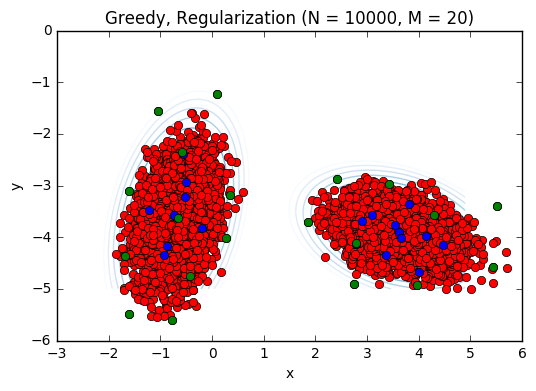
\includegraphics[width=\textwidth]{OriginalGaussian_20_2g_reg}
			\caption[Network2]%
			{{\small Network 1}}    
			\label{fig:mean and std of net14}
		\end{subfigure}
		\hfill
		\begin{subfigure}[b]{0.475\textwidth} 
			\centering 
			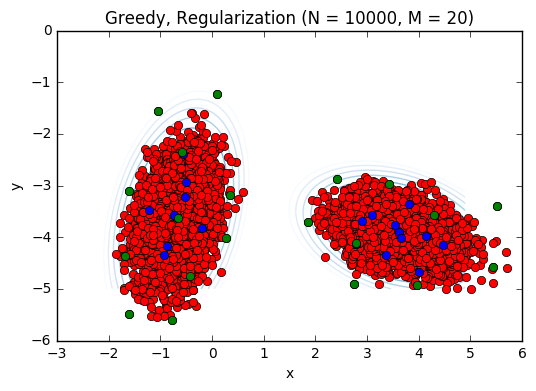
\includegraphics[width=\textwidth]{OriginalGaussian_20_2g_reg}
			\caption[]%
			{{\small Network 2}}    
			\label{fig:mean and std of net24}
		\end{subfigure}
		\vskip\baselineskip
		\begin{subfigure}[b]{0.475\textwidth}   
			\centering 
			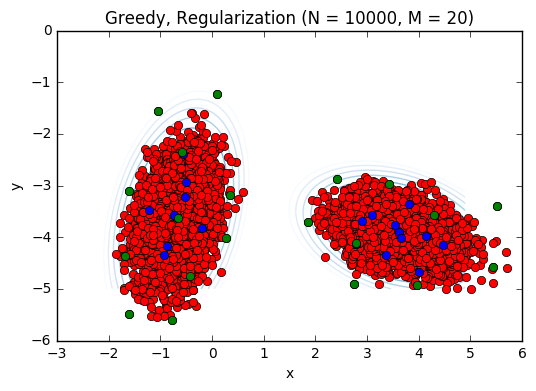
\includegraphics[width=\textwidth]{OriginalGaussian_20_2g_reg}
			\caption[]%
			{{\small Network 3}}    
			\label{fig:mean and std of net34}
		\end{subfigure}
		\quad
		\begin{subfigure}[b]{0.475\textwidth}   
			\centering 
			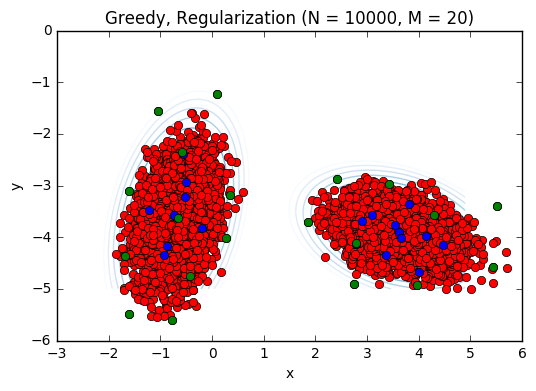
\includegraphics[width=\textwidth]{OriginalGaussian_20_2g_reg}
			\caption[]%
			{{\small Network 4}}    
			\label{fig:mean and std of net44}
		\end{subfigure}
		\caption[ The average and standard deviation of critical parameters ]
		{\small The average and standard deviation of critical parameters: Region R4} 
		\label{fig:mean and std of nets}
	\end{figure*}
	
	
	%\bibliographystyle{unsrt}
	\bibliographystyle{apalike}
	\bibliography{references}
	
\end{document}
